%
% This is Chapter 1 file (chap1.tex)
%
\chapter{UX Quality Assurance}
A self-critique of the UX for the final project of CISC472. Hosted versions of the project can be found at:

https://banningcalvin-redchan.glitch.me/

and at :

https://github.com/banningcalvin/redchan/.

It is important to note that because I created this, some level of bias may be present in that I knew my own design goals and built the design in a way that I was satisfied with. I am not entirely sure how others will interpret the layout or color scheme.
\section{Overview}


On the following pages is a series of screenshots for reference. In order, they are the homepage, the /a/ board, the /t/ board, and the account page.
\\\\
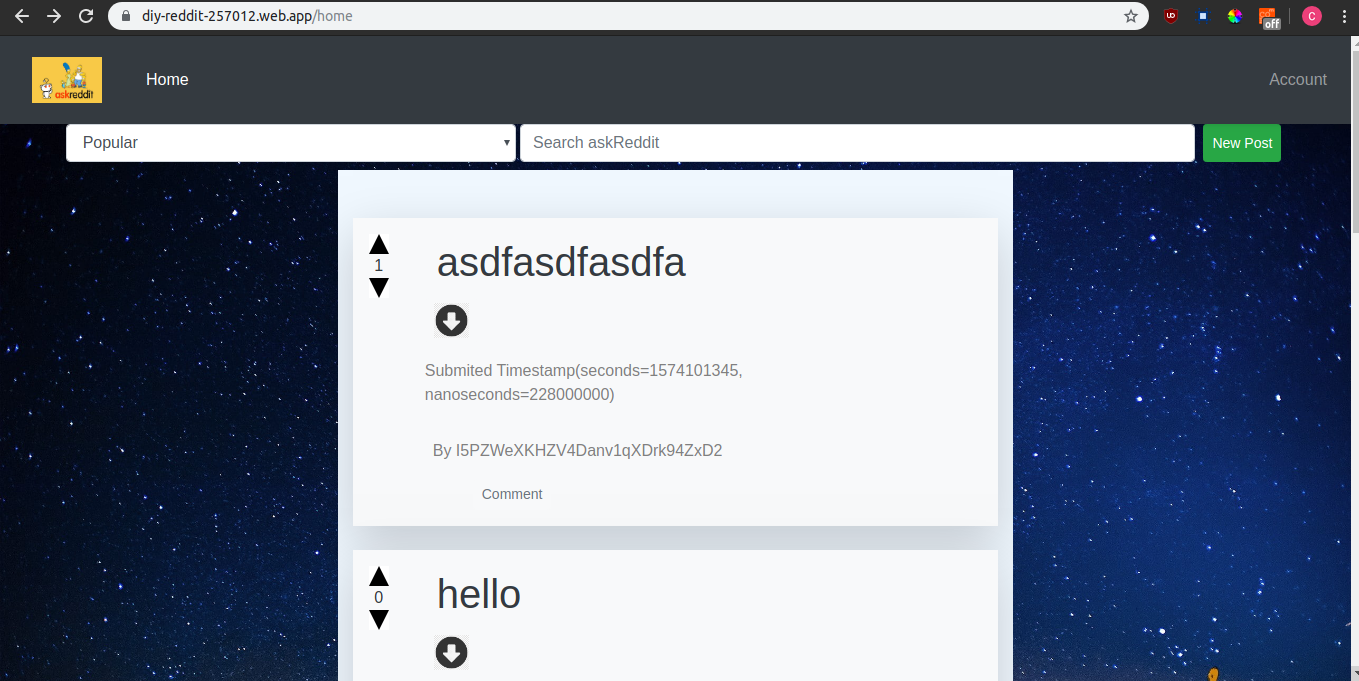
\includegraphics[width = 200pt]{images/home.png}
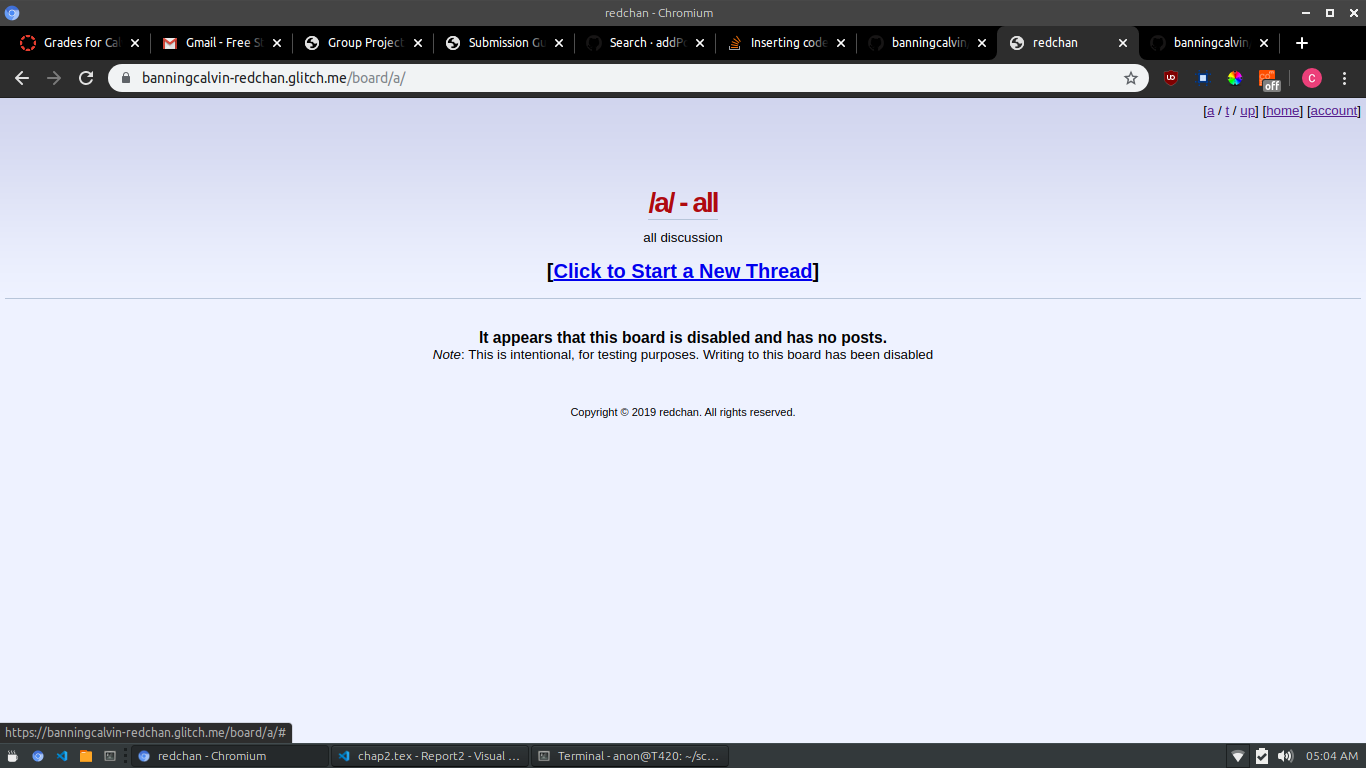
\includegraphics[width = 200pt]{images/aboard.png}
\\\\
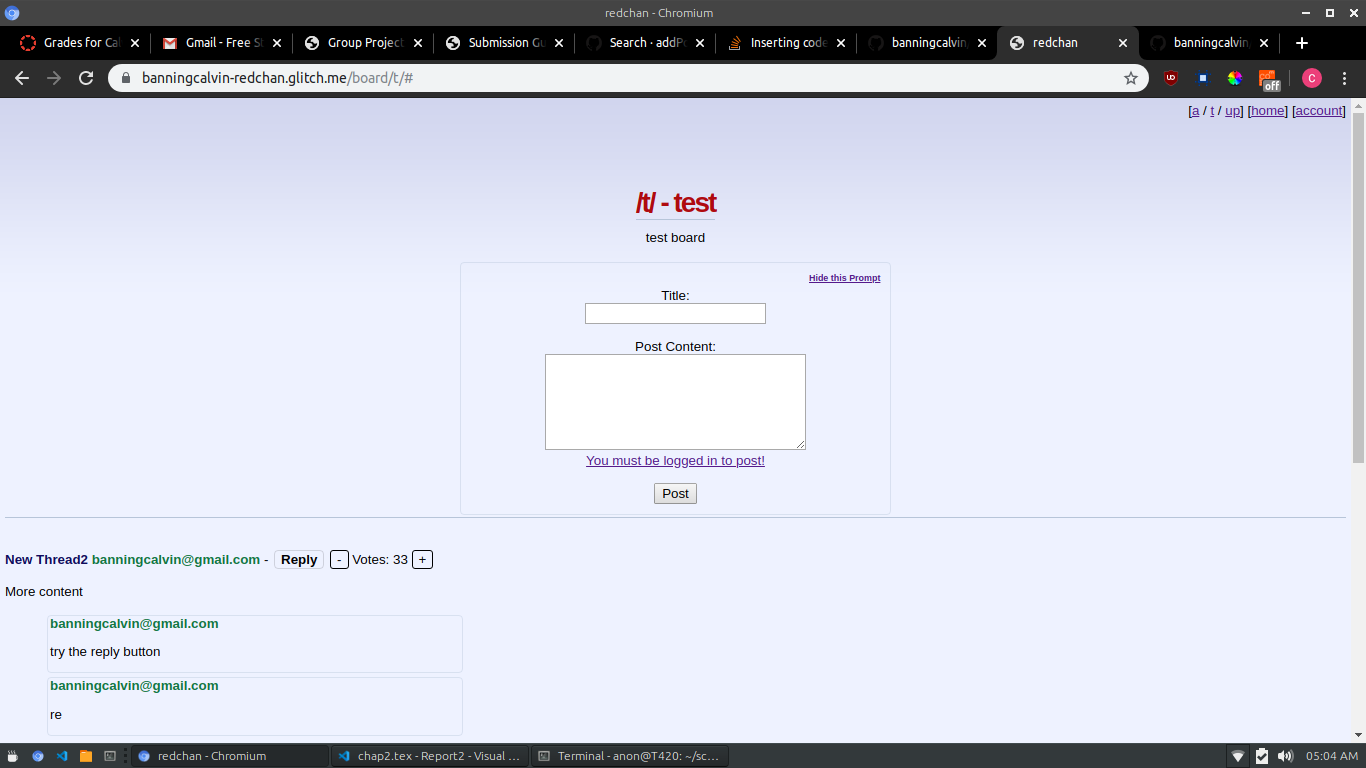
\includegraphics[width = 200pt]{images/tboard.png}
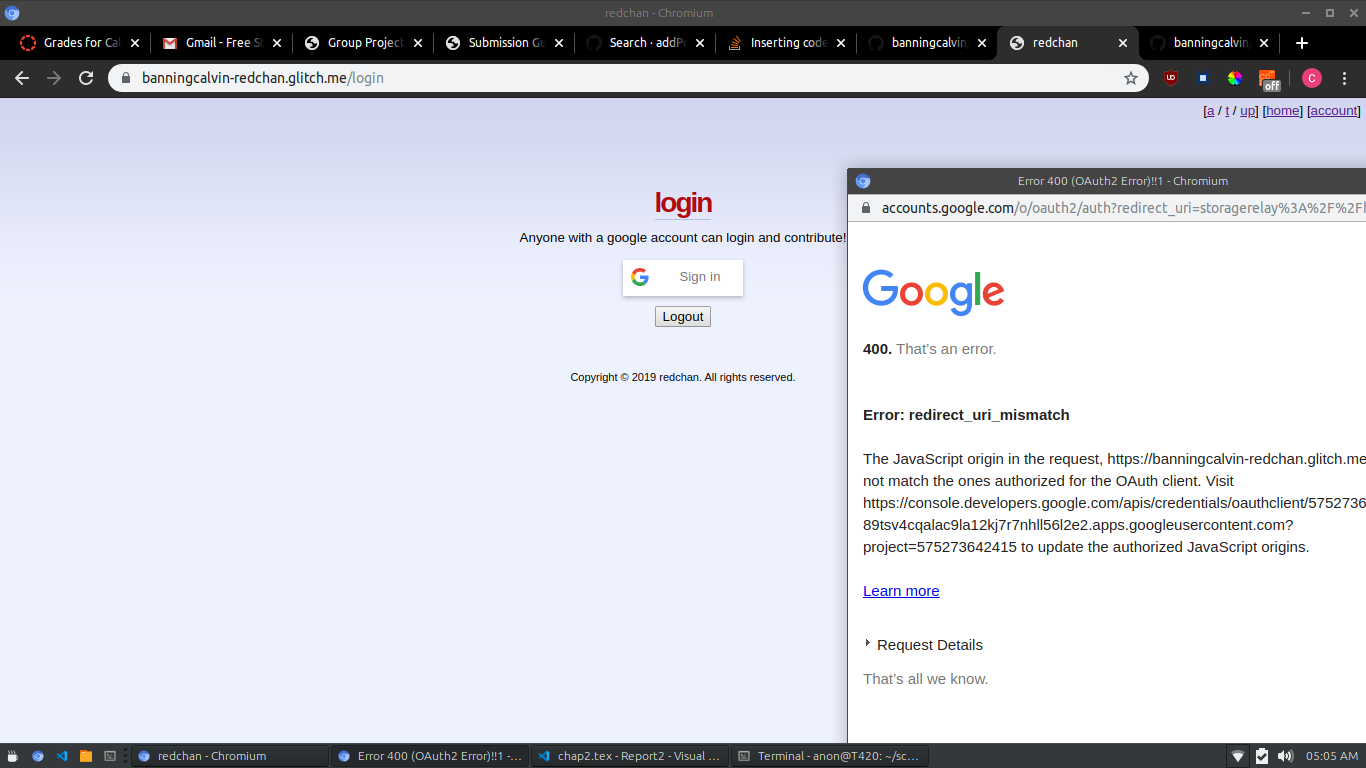
\includegraphics[width = 200pt]{images/account.png}
\\\\

\section{Evaluation}
The website clearly follows in the design of discussion boards less reputable than Reddit such as 4chan and 2chan. The site is not modern and does not follow modern design styles (as intended), but it does not fail to deliver an enjoyable and intuitive user experience.

The homepage delivers basic information: it offers links to the various boards, a link to the account page, and a message from the site owner. Having a dedicated homepage is justified to act as a sort of directory and noticeboard for the site, and helps give the site some character. Because the user experience is primarily derived from discussion, rather than from consumption, I felt that this character was refreshing.

The boards are straightforward in their purpose and navigation. The styling doesn't seem quite as perfected and uniform as the sites it's modelled after, but it seems to do 'enough'.

The login page isn't as clean as the rest of the site. The logout button is always shown, even when the user is logged out, and the login button is awkwardly situated in the middle of the screen.
\\\\
Other than that, the only other content on the site is posts. The /a/ board is disabled, but it has a notice which is professionally attached.

\section{Suggestions}
Not all users will share the admiration for this design style. In the same way that Reddit offers old.reddit.com, it might be useful to move this domain to old.redchan.com, and create a new frontend hosted at a different subdomain, which follows modern design fads. It should be understandable that this is out of scope for this project, as other tasks hold higher priority.

It would be wise to tweak the login and logout links to match the style of other buttons and links on the site. Additionally, the logout button should be displayed conditionally depending on the auth state.

On a final pass of the site, I discovered that upvotes were not working as expected. See chapter 1 for an overview on this bug and a suggested fix.
